Processes for DM annihilating into SM particles is depicted in fig. \ref{pic_annihilation}. So as for $b\rightarrow s \bar\mu\mu$, all model parameters are taken into
account
\begin{align}
 \left\{m_\chi, M_l, M_q, g^l_2\right\}
\end{align}
For $\chi$ being a Majorana fermion already implies that its s-wave cross section into a fermion pair is helicity suppressed and 
thus the leading contribution is p-wave \cite{1307.8120}. This can be explained as follows considering charge ($C$) and parity ($P$) symmetries.
The respective transformations for a fermion/antifermion state are ($C=(-1)^{L+S},\,P=(-1)^{L+1}$) with the total spin $S$ and the total orbital angular
momentum $L$. 
In the Majorana case $C=+1$. Moreover, s-wave means $S=0$ and hence $P=-1$. The $\bar f f$ state has to be able to reproduce the same $J=|L\pm S|$ 
which only has $S=0$ when the fermion and the antifermion are different Weyl spinors, i.e. both, fermion and antifermion are left-handed.
In chiral models like ours, in the limit of zero quark mass, we have $S=1$ giving $C=(-1)^{L+1},\,P=(-1)^{L+1}$ and therefore $C$ and $P$ are not 
conserved for any $L$. Hence, for s-wave annihilation a helicity flip, as for the anomalous magnetic moment of the muon, proportional to $m_f^2$ is 
required. Despite the fact that the muon is very light, it has an anticipated large coupling, above unity. The top quark has a coupling of order unity
but also a large mass. So we expect leading contributions for the annihilation from these two particles shaping the final state.
\begin{figure}[t]
 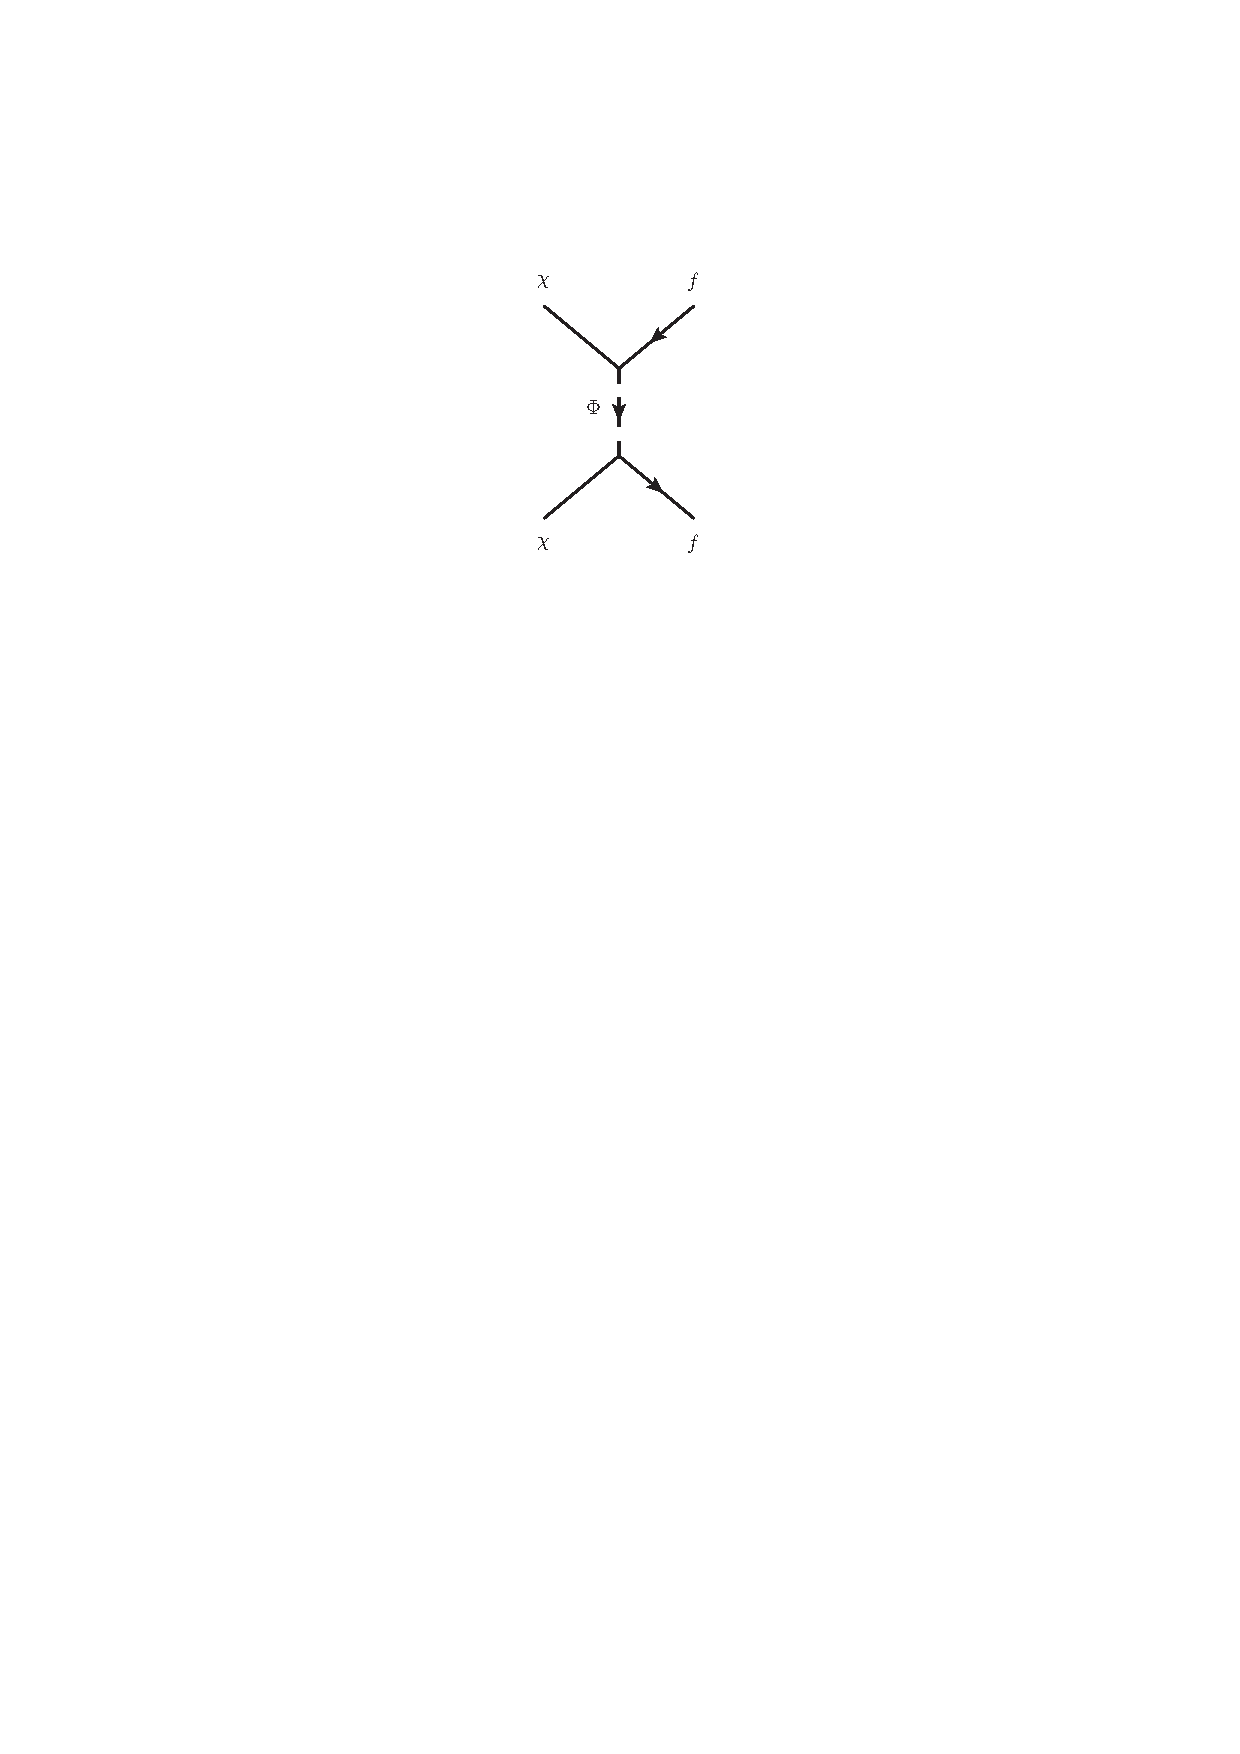
\includegraphics[width=1\textwidth]{../pics/ann.pdf}
 \caption{Annihilation processes for the neutral $\chi$ state into SM particles. The fermionic channel is dominant for muons and tops for both 
 representations. In case of a non-trivial isospin representation, the annihilation into $W$ bosons is enabled at tree-level. 
 SM bosons are characterised by $V$.}
 \label{pic_annihilation}
\end{figure}
% $VV$ annihilation (9207234), wino RD from other su2-states (0913-main)
% \begin{align}
%  \langle \sigma v \rangle^\text{D} \left(\bar \chi \chi \rightarrow \bar f f\right) = \frac{N_c g_f^4 m^2}{32\pi^2\left(M_l^2 + m^2\right)^2}
% \end{align}
The thermally averaged annihilation cross section into fermions is independent of the NP field representations \cite{1503.01500}
\begin{align}
 \langle \sigma v \rangle \left(\bar \chi^0 \chi^0 \rightarrow \bar f f\right) = \frac{N_c g_f^4}{32\pi m_\chi^2\left(1+x_f\right)^2} \left(\frac{m_f^2}{m_\chi^2} + \frac{2\left(1+x_f^2\right)}{3\left(1+x_f\right)^2} v^2\right)  .
\end{align}
For bosons there is no helicity or velocity suppression at leading order, but since the DM candidate carries almost no SM QN, decaying into vector
particles, such as photons, is loop suppressed. However, for the triplet there is an additional tree level decay into $W$-bosons which is, in some 
region, roughly as dominant as the decay into muons, depending on its coupling. The cross section reads\cite{1401.6212}
\begin{align}
 \langle \sigma v \rangle \left(\bar \chi^0 \chi^0 \rightarrow W^+W^-\right) = \frac{8\pi \alpha_2^2}{m_\chi^2} \frac{(1-w)^{\sfrac32}}{(2-w)^2}.
\end{align}
No co-annihilations are considered here for assumed non-degeneracy of $m_\chi$ and $M_{l,q}$. The velocity $v$ at the time when DM decoupled is
estimated as $v\approx 0.3$. 
%Nowadays $2\rightarrow3$ processes as $\bar \chi \chi \rightarrow \bar f f V$ might dominate with lower velocities 
%$v\approx 10^{-3}$, interesting for indirect detection \cite{1207.1431}. 